%-----------------------------------------------
% Template para criação de resumos de projectos/dissertação
% jlopes AT fe.up.pt,   Fri Jul  3 11:08:59 2009
%-----------------------------------------------

\documentclass[9pt,a4paper]{extarticle}

%% English version: comment first, uncomment second
%\usepackage[portuguese]{babel}  % Portuguese
\usepackage[english]{babel}     % English
\usepackage{graphicx}           % images .png or .pdf w/ pdflatex OR .eps w/ latex
\usepackage{times}              % use Times type-1 fonts
\usepackage[utf8]{inputenc}     % 8 bits using UTF-8
\usepackage{url}                % URLs
\usepackage{multicol}           % twocolumn, etc
\usepackage{float}              % improve figures & tables floating
\usepackage[tableposition=top]{caption} % captions
%% English version: comment first (maybe)
%\usepackage{indentfirst}        % portuguese standard for paragraphs
%\usepackage{parskip}

%% page layout
\usepackage[a4paper,margin=30mm,noheadfoot]{geometry}

%% space between columns
\columnsep 12mm

%% headers & footers
\pagestyle{empty}

%% figure & table caption
\captionsetup{figurename=Fig.,tablename=Tab.,labelsep=endash,font=bf,skip=.5\baselineskip}

%% heading
\makeatletter
\renewcommand*{\@seccntformat}[1]{%
  \csname the#1\endcsname.\quad
}
\makeatother

%% avoid widows and orphans
\clubpenalty=300
\widowpenalty=300

\begin{document}

\title{\vspace*{-8mm}\textbf{\textsc{Modelo de Escrita de Resumos de\\Projecto/Dissertação: um Exemplo}}}
\author{\emph{António Manuel Silva}\\[2mm]
\small{Projecto/Dissertação realizado sob a orientação do \emph{Prof.\ José Marco Soares}}\\
\small{na \emph{FazSoft Lda}}}
\date{}
\maketitle
%no page number
\thispagestyle{empty}

\vspace*{-4mm}\noindent\rule{\textwidth}{0.4pt}\vspace*{4mm}

\begin{multicols}{2}

\section{Motivação}\label{sec:motiva}

Neste documento apresentam-se alguns conselhos e instruções para a preparação dos resumos de projecto/dissertação.
Pede-se aos autores o favor de, dentro do possível, cumprirem com as instruções que são dadas, assim como com a estrutura apresentada, de forma a manter-se o mesmo aspecto em todos os resumos.
Nas sub-secções~\ref{sec:lingua} a ~\ref{sec:number} podem encontrar-se alguns detalhes sobre a formatação do documento.

Na secção ``Motivação'' deve ser apresentado o enquadramento do trabalho, dando ideia das necessidades que o mesmo cobre.

\section{Objectivos}\label{sec:goals}

A secção ``Objectivos'' deve enunciar claramente os objectivos a atingir com o trabalho de projecto/dissertação, enquadrando-os na respectiva área de actividade a que o trabalho se destina.
Por exemplo, este documento tem como objectivos:
\begin{itemize}
\item Servir de modelo/exemplo do ponto de vista da dos resumos;
\item Apresentar o aspecto gráfico que se pretende para os resumos;
\item Disponibilizar \emph{templates} a quem pretenda utilizar \LaTeX.
\end{itemize}

\section{Descrição do Trabalho}\label{sec:work}

Na secção ``Descrição do Trabalho'' (com este ou com outro nome que se julgue mais adequado) devem ser apresentadas as principais partes do trabalho, começando pela sua estruturação. Devem ser mencionadas as tecnologias utilizadas, com referências à sua interdependência e interligação dando especial ênfase aos componentes desenvolvidos pelo estudante no âmbito do trabalho em causa.

No presente documento, seguem-se 9 subsecções com instruções acerca da extensão da comunicação, margens, estilos e outras recomendações gerais acerca da elaboração da versão final dos resumos.

\subsection{Línguas Obrigatórias}\label{sec:lingua}

Os resumos deverão ser apresentados, em ficheiros separados, em versões portuguesa e inglesa.
No resumo em Português e em caso de necessidade de utilização de termos em língua Inglesa, estes deverão ser devidamente salientados pela adopção da fonte em itálico, como, por exemplo, \emph{Ray-Tracing}.

\subsection{Cabeçalho de Identificação}

O cabeçalho de identificação deve ser centrado e inicia-se com o título da comunicação, em letras maiúsculas de tamanho 12 e em negrito.
Seguem-se, em linhas separadas e em tamanho 9, a identificação do estudante, da empresa e dos orientadores (estes dois numa única linha).
Todos os quatro nomes devem ser em itálico.

\subsection{Extensão do Artigo e Tipo de Letra}

Cada resumo deve ser formatado com texto a duas colunas, não devendo exceder duas páginas de formato A4.
\textbf{As duas colunas devem terminar sensivelmente à mesma altura}, em cada uma das páginas.

O tipo de letra para o texto genérico deverá ser \emph{Times New Roman} com tamanho 9 e espaçamento simples entre linhas.
O espaçamento entre parágrafos deverá ser estendido a 1.5 linhas (0.5 linha de espaçamento extra).

\subsection{Dimensões das Margens}

As margens a manter à volta do texto deverão ser as constantes na Tab.~\ref{tab:medidas}.

\begin{table}[H]
  \centering
  \caption{Margens expressas em centímetros}
\begin{tabular}{c | c}
	\hline
\textbf{Espaçamento} & \textbf{Medida}\\
	\hline
	\hline
        Margem Superior & 3 cm\\
        Margem Inferior & 3 cm\\
        Margem Esquerda & 3 cm\\
        Margem Direita  & 3 cm\\
        Entre Colunas   & 1.2 cm\\
	\hline
\end{tabular}
  \label{tab:medidas}
\end{table}

\subsection{Corpo do Texto}

Todos os títulos de secções e subsecções devem ser escritos em negrito e com um espaçamento para cima ligeiramente superior ao de um parágrafo normal.
Os títulos de níveis um e dois devem ter tamanhos, respectivamente, 11 e 9.
As ``subsubsecções'' devem ser evitadas.

\subsection{Numeração das Secções}

As secções deverão ser numeradas com início em "1", de acordo com os níveis e subníveis respectivos, usando-se o ponto como separador.

\subsection{Figuras, Equações e Quadros}

As figuras e as tabelas deverão ser centradas, sempre que possível, à largura da coluna de texto em que se
inserem (Tab.~\ref{tab:medidas} e Fig.~\ref{fig:figura}).
As figuras e tabelas cujas dimensões não o permitam, podem ser centradas à largura da página.

\begin{figure}[H]
\centerline{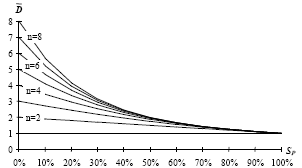
\includegraphics[scale=.6]{figura.png}}
\caption{Esta é a legenda da figura}
\label{fig:figura}
\end{figure}

As legendas das figuras, a negrito, devem ser colocadas na sua parte inferior, contendo a respectiva numeração antecedida do termo \textbf{Fig.}
O mesmo é aplicável às tabelas, excepto que a legenda deve ser iniciada pelo termo \textbf{Tab.}\ e deve ser colocada acima da tabela respectiva.
Devem ser evitadas figuras ou outros elementos com cores.

\begin{equation}
  S_{L,i} = S_{L,i-1} . (1-S_{P,i-1}) = \prod_{k=0}^{i-1} (1-S_{p,k}) \label{eq:cif}
\end{equation}
% \begin{eqnarray}
% S_{L,i} &=& S_{L,i-1} . (1-S_{P,i-1}) \nonumber\\
%        &=& \prod_{k=0}^{i-1} (1-S_{p,k}) \label{eq:cif}
% \end{eqnarray}

As equações deverão conter a respectiva numeração na mesma linha de texto e à sua direita, entre parêntesis, como se mostra no exemplo da Equação~\ref{eq:cif}.

As figuras deverão ser numeradas a partir do número 1 e com uma única sequência, i.e., sem reinício em cada secção.
O mesmo deve suceder com as equações e com as tabelas.

\subsection{Numeração de Páginas}\label{sec:number}

As páginas \textbf{NÃO} devem ser numeradas.

\subsection{Codificação dos Caracteres}\label{sec:encomding}

Este exemplo está escrito em UTF-8; para outras codificações deverá
ser alterado \texttt{\\usepackage[utf8]\{inputenc\}}.


\section{Conclusões}\label{sec:conclui}

Espera-se que este documento possa contribuir para uma melhor qualidade dos resumos dos projectos/dissertações do MIEIC/FEUP.

Documentos que não respeitem este aspecto gráfico serão liminarmente recusados, ficando os respectivos autores em falta em relação à sua entrega.

Para as dissertações existem regras definidas noutro lado~\cite{kn:Mat93}.

%%English version: comment first, uncomment second
%\bibliographystyle{unsrt-pt}  % numeric, unsorted refs
\bibliographystyle{unsrt}  % numeric, unsorted refs
\bibliography{refs}

\end{multicols}

\end{document}
